%Copyright 2021 Jean-Michel Bruel
%This program is free template, under the terms of the attached License of this repo. 
%Based on https://github.com/jpeisenbarth/SRS-Tex
%Itself based on the code of Yiannis Lazarides
%http://tex.stackexchange.com/questions/42602/software-requirements-specification-with-latex
%http://tex.stackexchange.com/users/963/yiannis-lazarides
%Also based on the template of Karl E. Wiegers
%http://www.se.rit.edu/~emad/teaching/slides/srs_template_sep14.pdf
%http://karlwiegers.com
\documentclass{scrreprt}
\usepackage{method}		% Specific command from Handbook
\usepackage{minitoc}	% For table of content in chapters
\usepackage{listings}
\usepackage{underscore}
\usepackage{xcolor}
\usepackage{booktabs}
\usepackage{makecell}
\usepackage{graphicx}
\usepackage{float}
\usepackage{tabularx}
\usepackage[bookmarks=true]{hyperref}
\usepackage[utf8]{inputenc}
\usepackage[english]{babel}
\hypersetup{
    bookmarks=false,    % show bookmarks bar?
    pdftitle={Software Requirement Specification - Room8},    % title
    pdfauthor={Mohammed Abed, Maged Armanios, Jinal Kasturiarachchi, Jane Klavir, Harshil Patel},                     % author
    pdfsubject={TeX and LaTeX},                        % subject of the document
    pdfkeywords={TeX, LaTeX, graphics, images}, % list of keywords
    colorlinks=true,       % false: boxed links; true: colored links
    linkcolor=blue,       % color of internal links
    citecolor=black,       % color of links to bibliography
    filecolor=black,        % color of file links
    urlcolor=purple,        % color of external links
    linktoc=page            % only page is linked
}%
\def\myversion{0.0.0}
\date{}
%\title
\usepackage{hyperref}
\newcommand*{\nsection}[1]{
    \section*{#1}
    \addcontentsline{toc}{section}{#1}
}

\newcommand*{\nsubsection}[1]{
    \subsection*{#1}
    \addcontentsline{toc}{subsection}{#1}
}
%--------------------- Numbering ---------------
\usepackage{amsthm}
\usepackage{xassoccnt}
%\newtheorem{req}{Requirement}[section]        
\newtheorem{req}{Requirement}        
\theoremstyle{definition}        
\newtheorem{constraint}{Constraint}
\newtheorem{goal}{Goal}
\newtheorem{benefit}{Benefit}
\newtheorem{limitation}{Limitation}
\newtheorem{exclusion}{Exclusion}
\DeclareCoupledCountersGroup{theorems}
\DeclareCoupledCounters[name=theorems]{req,constraint,goal}
\setcounter{goal}{0}
%--------------------- Comments ---------------
\newcommand{\mynote}[3][black]{\textcolor{#1}{\fbox{\bfseries\sffamily\scriptsize{#2}}
{\small\textsf{\emph{#3}}}}}
\newcommand{\comment}[1]{\mynote[red]{Comment:}{#1}}
%\newcommand{\comment}[1]{}
\newcommand{\notEmpty}{\comment{This chapter should not be empty!}}

\begin{document}

\begin{center}
    \rule{16cm}{5pt}\vskip1cm
    \begin{bfseries}
        \Huge{SOFTWARE REQUIREMENTS\\ SPECIFICATION}\\
        \vspace{1.9cm}
        Room8\\
        \vspace{1.9cm}
        \LARGE{Version \myversion}\\
        \vspace{1.9cm}
        Prepared by:\\
        Mohammed Abed\\ 
        Maged Armanios\\
        Jinal Kasturiarachchi\\
        Jane Klavir\\
        Harshil Patel\\
        \vspace{0.9cm}
        McMaster University\\
        \vspace{0.9cm}
        \today\\
    \end{bfseries}
\end{center}

%===============================================================
\chapter*{Revision History}
%===============================================================

\begin{center}
    \begin{tabular}{|c|c|c|c|}
        \hline
        Name        & Date          & Reason For Changes & Version\\
        \hline
        \hline
        \makecell{Mohammed A. \\ Maged A. \\ Jinal K. \\ Jane K. \\ Harshil P.} & 2024-10-11 & First Draft & 0.0\\
        \hline
        \makecell{Mohammed A.} & 2024-11-04 & Added FR225 for ChatBot & 0.1\\
        \hline
    \end{tabular}
\end{center}

This document follows the requirements documentation structure presented in the \href{ https://link.springer.com/content/pdf/10.1007/978-3-031-06739-6.pdf}{Handbook of requirements and business analysis}, by Bertrand Meyer.

%===============================================================
\dominitoc% Initialization
\tableofcontents
\adjustmtc
%===============================================================

%===============================================================
\addcontentsline{toc}{chapter}{Goals book}
\chapter*{Goals}

\minitoc% Creating an actual minitoc
%===============================================================

\nsection{G.1 Context and overall objective}
%---------------------------------
\begin{flushleft}
Shared living environments often create tension between roommates. It is usually cumbersome to reach out to a roommate about messes they left behind in a shared space, concerns over bill payments, household upkeep, and more. Our project, Room8, aims to prevent these cumbersome interactions by providing an application and the necessary hardware components to help monitor the cleanliness of shared spaces, schedule tasks, track shared billing cycles, and alert roommates of any issues within the shared house.
\end{flushleft}

\begin{goal}\label{goal:first}
Create a system that monitors the cleanliness of a shared living space, such as a kitchen or a living room.
\end{goal}
\begin{goal}\label{goal:second}
Provide roommates with a centralized platform to manage, schedule, and task household tasks.
\end{goal}
\begin{goal}\label{goal:third}
Provide roommates with a centralized platform to manage, schedule, and track bill payments.
\end{goal}
\begin{goal}\label{goal:fourth}
Alert and remind roommates of issues regarding issues related to the shared living spaces, reducing tension between each other.
\end{goal}

\nsection{G.2 Current situation}
%---------------------------------
\begin{flushleft}
Room8 is designed to reduce points of tension and reduce the need for frustrating dialogue commonplace with people in shared housing, especially students. Currently, in order to manage the many shared responsibilities, roommates have to utilize multiple techniques or tools such as physical calendars, notification reminders, and existing applications such as Splitwise which do not have any integrations between each other. Additionally, it is estimated that approximately 25\% students experience conflicts with a roommate, harming academic performance and inducing stress [1]. Recognizing these factors, Room8 aims to create a centralized platform that not only simplifies communication but reduces stress and conflict to improve the lives of students. 
\end{flushleft}

\nsection{G.3 Expected benefits}
%---------------------------------
\begin{flushleft}
As stated in section G.2, conflicts between roommates create more than issues in the home and involve more than just misunderstandings in scheduling tasks or living standards. By creating a centralized suite that will help roommates monitor, schedule, and coordinate, Room8 will reduce conflicts between roommates over misunderstandings and miscommunications, and allow for greater flexibility in assigning responsibilities. Additionally, reduced conflicts will lead to mental health benefits for those living in the home by lowering conflict-related stress.  Finally, Room8 is expected to improve academic performance in some students who are hindered academically by conflicts with roommates (approximately 17\% of students [1]). 

\begin{benefit}\label{benefit:first}
An improvement in response times amongst roommates over household concerns.
\end{benefit}

\begin{benefit}\label{benefit:first}
Increased flexibility in task scheduling and management, due to the presence of a centralized application.
\end{benefit}

\begin{benefit}\label{benefit:first}
Improved communication and transparency over household matters between roommates.
\end{benefit}

\begin{benefit}\label{benefit:first}
A reduction of events in which a roommate forgets or neglects their responsibilities to the home.
\end{benefit}

\begin{benefit}\label{benefit:first}
Improved household cleanliness and upkeep.
\end{benefit}

\begin{benefit}\label{benefit:first}
A reduction in conflicts between roommates over household matters.
\end{benefit}

\begin{benefit}\label{benefit:first}
A reduction in stress for roommates due to reduced conflicts amongst each other.\end{benefit}

\begin{benefit}\label{benefit:first}
Improved mental health for students who experience conflicts with roommates.
\end{benefit}

\begin{benefit}\label{benefit:first}
An improvement in academic performance for students experience stress caused by issues with roommates.
\end{benefit}

\end{flushleft}

\nsection{G.4 Functionality overview}
%---------------------------------
\begin{flushleft}
    \item \textbf{User \& House Management:} The system allows students to register, create, and manage their accounts. Students are also able to create homes and invite other students. 
    
    \item \textbf{Cleanliness Management:} Students are able to set up cameras in their shared living spaces. Machine learning algorithms are used to detect messes and assign them to the students to increase accountability and to reduce communication friction. 
    
    \item \textbf{Scheduler:} The system allows users to create and manage chore and cleaning schedules. It will also send reminders to users about their assigned chores and cleaning tasks. Additionally, users are able to "book" common areas that are available within the shared space (i.e. party room, study room, etc.) to avoid conflicts 
     
    \item \textbf{Bill Splitter:} Students are able to add shared expenses to the house and keep track of who owes what. The system will automatically split the bills between the chosen students. 

    \item \textbf{Chat:} The system provides an exportable ChatBot to SMS group chats to aid in home management and communication. The ChatBot will be able to send reminders and notifications to the group chat about upcoming events, chores, and bills.
    
    \item \textbf{Compliance and Data Privacy:} The system follows data privacy and compliance with Personal Information Protection and Electronic Documents Act (PIPEDA), Ontario’s Freedom of Information and Protection of Privacy Act (FIPPA), and Anti-Spam Legislation (CASL) to ensure that students' data is secure and not shared with third parties.
    
    \item \textbf{Progressive Web App:} The system is hosted as a progressive web app (PWA), so users can use it on their phones and computers.
\end{flushleft}

\nsection{G.5 High-level usage scenarios}
%---------------------------------
\begin{figure}[H]
    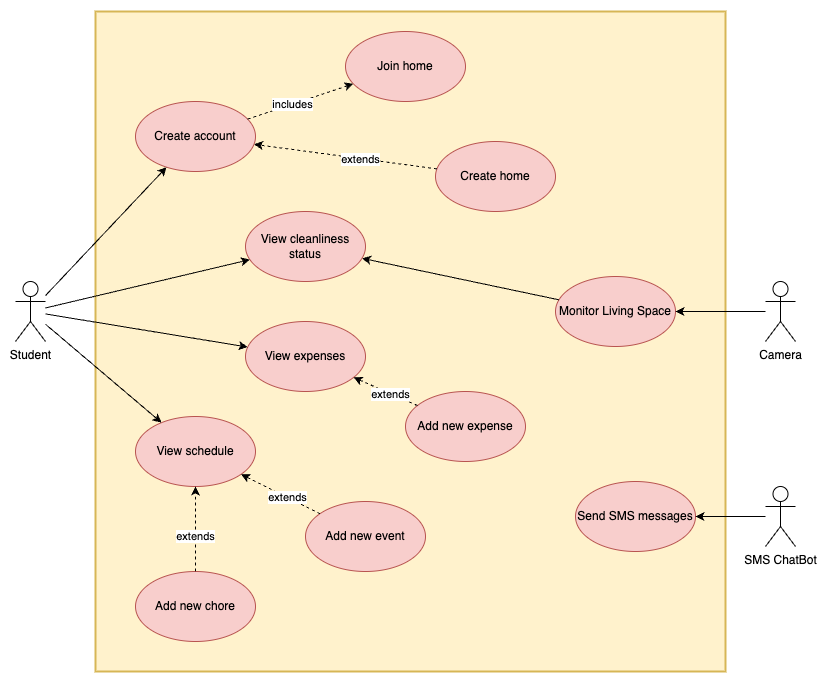
\includegraphics[width=\linewidth]{./img/use-case-diagram.png}
    \caption{High level use case diagram}
    \label{fig: High level use case diagram}
\end{figure}

\begin{itemize}
    \item UC1: Account Management
    \begin{enumerate}
        \item User accesses the Room8 app.
        \item User selects "Create Account" or "Log In".
        \item User fills in personal information (name, email, password).
        \item User submits the form.
        \item System validates the information and authenticates the account.
        \item System redirects the user to their dashboard.
    \end{enumerate}  
    
    \item UC2: Home Management
    \begin{enumerate}
        \item User navigates to their dashboard.
        \item User selects the "Create Home" or "Join an Existing Home" option.
        \item User enters home details (home name, address, etc.).
        \item User sends invitations to housemates by entering their email addresses.
        \item System sends email notifications to invited users.
        \item Invited users accept or decline the invitation.
    \end{enumerate}
    
    \item UC3: Schedule Manager
    \begin{enumerate}
        \item User navigates to the "Schedule” section.
        \item User selects "Add New Chore" or "Add New Event".
        \item User inputs chore details (name, description, time, frequency, assigned users, etc.).
        \item System saves the chore and sends reminders to the assigned users.
        \item Users are able to view the schedule and mark chores as complete.
    \end{enumerate}
    
    \item UC4: Bill Splitter
    \begin{enumerate}
        \item User navigates to the “Bill Splitter” section.
        \item User selects the "Add Expense" option.
        \item User enters the total expense amount and description.
        \item User selects which housemates are responsible for the expense.
        \item System splits the expense and notifies the involved users.
        \item Users are able to view the total expenses and who owes what.
        \item Users are able to mark expenses as paid.
    \end{enumerate}
    
    \item UC5: Cleanliness Management
    \begin{enumerate}
        \item User navigates to the “Cleanliness Management” section.
        \item System displays the current cleanliness score and detected messes.
        \item User selects another user to view their cleanliness score.
        \item System displays the selected user’s cleanliness score and pending tasks.
    \end{enumerate}
    
    \item UC6: SMS ChatBot
    \begin{enumerate}
        \item User navigates to the “Chat Management” section.
        \item User selects the option to add a ChatBot to their house group chat.
        \item User inputs notification and reminder settings.
        \item System generates an SMS numbers and instructions to add the ChatBot to the group chat.
        \item The ChatBot sends a welcome message to the group.
        \item The ChatBot sends notifications and reminders to the group chat.
    \end{enumerate}
    
\end{itemize}
    
\nsection{G.6 Limitations and exclusions}
%---------------------------------
Below is a list of limitations and exclusions the system will not address:
\begin{limitation}\label{limitation:first}
System will not track activity completed by the user in the shared environment.
\end{limitation}
\begin{exclusion}\label{exclusion:first}
System will not request or send money directly to users in the bill splitting functionality.
\end{exclusion}
\begin{exclusion}\label{exclusion:second}
System will not use images taken to train machine learning model.
\end{exclusion}

\nsection{G.7 Stakeholders and requirements sources}

\begin{table}[ht]
\centering
\begin{tabular}{|l|l|}
\hline
\textbf{Stakeholder} & \textbf{Category} \\ \hline
Students              & Direct  \\ \hline
Landlords and Residence Assistants         & Indirect \\ \hline
University Housing Committee & Indirect \\ \hline
\end{tabular}
\caption{Stakeholders and Categories}
\end{table}

\nsubsection{G.7.1 Direct Stakeholders}
\textbf{Students Off Campus} \\ Students off campus are the primary direct stakeholders for Room8. They are the main users of the mobile application who create houses within the app and set up the camera systems. These students seek to maintain cleanliness in their shared living spaces and establish accountability when a mess is left behind by a roommate. The application addresses common challenges faced by students in shared living arrangements, such as maintaining cleanliness, splitting expenses, and scheduling activities. \\
\\
\textbf{Students On Campus} \\ Students on campus are the other direct stakeholders for Room8. They are the main mainly concerned with the chore and activity scheduling aspect of the app. In most cases students living on campus do not have a kitchen and individuals are responsible for keeping their own rooms clean so these types of students would benefit from scheduling the cleaning of public spaces (eg. pool table, game space) and seeing events that are happening.

\nsubsection{G.7.2 Indirect Stakeholders}
\textbf{Landlords} \\ Landlords are the main indirect stakeholders to the project. Landlords are renting out their homes to students and are concerned with the condition their house is kept in. They are looking to maintain the clean condition of their home which is done by holding students accountable for messes that are made.\\
\\
\textbf{Residence Assistants} \\ Resident assistants are another indirect stakeholder who would benefit from Room8 specifically the activity scheduling feature. Resident assistants are responsible for hosting events for students living on campus and Room8 provides a calendar system to make events on a shared calendar to inform students of any upcoming activities.\\
\\
\textbf{University Housing Committee} \\ The University Housing Committee is another key indirect stakeholder in the project. These committees often seek to help students transition into living in shared spaces and provide guidance and support. Room8 offers a wide range of services that address common points of frustration faced by students, which are often brought up to these university committees. By facilitating better communication and organization, Room8 helps enhance the overall living experience for students.



%===============================================================
\chapter*{Environment}
\addcontentsline{toc}{chapter}{Environment book}
\setcounter{mtc}{2}
\minitoc% Creating an actual minitoc
%===============================================================


\nsection{E.1 Glossary}
The glossary provides definitions for the key terms used throughout the project. It includes terminology related to the system’s environment and functionality, ensuring that all parties involved have a clear understanding of the concepts and language specific to the project. This helps prevent miscommunication and fosters consistency in documentation and development.
\begin{flushleft}
    \item \textbf{SRS (Software Requirements Specification):} A formal document (this document) that outlines the functional and non-functional requirements of a system or software application. It serves as a blueprint for both developers and stakeholders, detailing what the system is expected to do, how it should perform, as well as assumptions/ constraints for its development.\newline

    \item \textbf{Room8:} The name of the application being described by this SRS. Room8 is an app designed to help students manage shared living spaces. It includes functionalities like cleanliness monitoring, chore scheduling, bill splitting, and communication tools to streamline household tasks.\newline

    \item \textbf{Home:} In the context of Room8, a "home" refers to the digital representation of a shared living space comprised of students. Essentially, it is the user group for one living space where all members can manage, organize, and recieve alerts for household responsibilities.\newline

    \item \textbf{Students:} In the context of Room8, a "student" is a user of the app. \newline

    \item \textbf{V\&V (Verification and Validation):} A process in software development aimed at ensuring that a system meets its specifications (verification) and that it fulfills its intended purpose (validation).\newline

    \item \textbf{Splitwise:} A real-world app used for tracking and splitting shared expenses between individuals.\newline

    \item \textbf{Chatbot:} Software designed to simulate conversation with users, often through text-based interaction. In Room8, the ChatBot automates tasks such as sending reminders, notifications, and facilitating communication about chores and bills in group chats.\newline

    \item \textbf{PIPEDA (Personal Information Protection and Electronic Documents Act):} A Canadian law governing how private sector organizations collect, use, and disclose personal information in the course of their business activities. Compliance ensures that user data is protected and handled with consent.\newline

    \item \textbf{FIPPA (Freedom of Information and Protection of Privacy Act):} A piece of Canadian legislation that outlines the rights of individuals to access government information and the responsibilities of public organizations to protect personal privacy. It helps ensure the secure handling of personal information.\newline

    \item \textbf{CASL (Canadian Anti-Spam Legislation):} A Canadian law aimed at regulating commercial electronic messages, including emails and texts, to prevent spam. It requires consent before sending such communications, ensuring transparency and privacy.\newline

    \item \textbf{"Before" Picture:} The image of the shared living space before a student enters and uses it.\newline

    \item \textbf{"After" Picture:} he image of the shared living space after a student uses it.\newline

    \item \textbf{CASL (Cleanliness Score):} A score assigned to a student after they have finished using the shared living space. It is derived from an algorithm in which the inputs are a "before" and "after" picture pair.\newline

    \item \textbf{OAuth 2.0:} An open standard protocol for authorization, allowing secure access to user data across different services without revealing login credentials. OAuth is commonly used to enable single sign-on or to grant third-party applications limited access to a user's resources.\newline

    \item \textbf{PPM (Pixels Per Metre):} A measurement used to define the resolution of digital images, specifically indicating the number of pixels within a meter of space. It is often used in imaging, mapping, and display technologies to describe the level of detail or clarity in an image.\newline

    \item \textbf{FoV (Field of View):} In digital images, FoV refers to the extent of the observable area at any given moment. It is the angle/ scope that the camera sees.\newline

    \item \textbf{UTC (Coordinated Universal Time):} A time standard used globally to regulate clocks and time. It is the primary time standard by which the world regulates time and is not affected by time zones or daylight saving changes. UTC is crucial for coordinating activities across different time zones, especially in computing, aviation, and telecommunications.\newline

    \item \textbf{JS (JavaScript):} A popular, lightweight programming language commonly used to build dynamic content on websites. JavaScript allows developers to create interactive web pages and web applications.\newline

    \item \textbf{TS (TypeScript):} A superset of JavaScript that introduces static types, making the code more robust and easier to debug. TypeScript is particularly helpful for large-scale applications by catching potential errors at compile time.\newline

    \item \textbf{AWS (Amazon Web Services):} A comprehensive cloud computing platform provided by Amazon, offering a wide range of services such as computing power, storage, databases, and machine learning. AWS enables scalable and secure cloud solutions for various applications.\newline

    \item \textbf{CI/CD (Continuous Integration and Continuous Deployment/Development):} A set of practices in software development aimed at automating and streamlining the process of integrating code changes (CI) and deploying applications (CD). CI/CD improves code quality, speeds up development cycles, and ensures faster delivery of new features or updates.\newline

    \item \textbf{PoC (Proof of Concept):} A prototype or small-scale experiment conducted to verify that an idea or technology is feasible. In software development, a PoC helps validate whether a particular solution or approach will work as intended before full-scale implementation.\newline

\end{flushleft}


\nsection{E.2 Components}
This section outlines the relevant external components that the system will interact with. These include existing systems or services, particularly software, that will provide or consume APIs. These interactions play a significant role in how the system operates within its broader ecosystem, impacting design and integration.
\begin{flushleft}
  \item \textbf{Motion-activated camera:} Room8 will be connected to a camera that is activated by motion in the shared space. This component is used for taking a “before” and “after” picture that serves as the input for the cleanliness detection model. \newline
  
  \item \textbf{Object detector API:} Room8 will utilize an object detector that performs on a pair of images (i.e. the “before” and “after” picture) taken by the motion-activated camera. Object detection enables the algorithm to quantify the difference in room states as a function of objects and their transformations.\newline 
  
  \item \textbf{Household items dataset:} The ML model will be pre-trained with a dataset containing common household and kitchen items. This will allow the object detector to classify the items it detects and is important for providing valuable output to students.\newline
   
  \item \textbf{Google calendar API:} Room8 will interface with Google calendar to facilitate scheduling chores and events. This is critical for Room8's chore scheduling.\newline

  \item \textbf{SMS ChatBot:} The application employs a ChatBot to send notifications to students via SMS about their responsibilities in the home (i.e. cleaning their mess from shared spaces, upcoming chore deadlines, and money owed for shared bills). This helps with bookkeeping, enforcing fairness, and keeping shared spaces clean.\newline

  \item \textbf{OAuth 2.0:} The app utilizes the OAuth 2.0 protocol to manage user authentication and authorization securely. OAuth 2.0 allows Room8 to provide a seamless login experience using third-party identity providers without requiring users to create and manage separate credentials. OAuth 2.0 handles the app’s legal and privacy compliance standards.\newline
  

\end{flushleft}

\nsection{E.3 Constraints}
Constraints are non-negotiable limitations imposed on the system, stemming from external factors such as business rules or technical requirements. These restrictions must be strictly adhered to during development. Constraints can influence system design and implementation, and their fulfillment is critical to ensuring the system meets its operational requirements.
%---------------------------------
\begin{flushleft}
  \item \textbf{Camera resolution:} The resolution of the motion-activated camera affects the quality of the input that is used by the object detector. Depending on the PPM of the image, there is a minimum viable object size for a given object to be classified.\newline
  
  \item \textbf{Platform compatibility:} The application must be compatible on Android and iOS to accommodate all users in the home.\newline 
  
  \item \textbf{Data privacy compliance:} The application adheres to all applicable data privacy regulations for the region in which it operates. User data must be handled with the utmost care and cannot be shared or used without explicit consent. Prior to collecting, storing, or processing any personal data, the appropriate permissions must always be obtained to ensure compliance with privacy laws and to respect user rights. \newline

\end{flushleft}
%---------------------------------


\nsection{E.4 Assumptions}
Assumptions are conditions that are presumed to be true during development to simplify system design. These are not externally enforced but are accepted for the sake of convenience or efficiency. While helpful, assumptions must be carefully evaluated, as changes in the assumed conditions could affect the system’s success or performance.
\begin{flushleft}
  \item \textbf{Network connectivity:} The application assumes that there is reliable internet connection. Operating under this assumption, the camera is able to transfer images to the detector and students have access to updated synchronized information when using the app.\newline

  \item \textbf{Operating system support:} The application is compatible with the versions of Android and iOS that are currently supported by mobile providers.\newline
  
  \item \textbf{Common household items dataset:} The classifier can assume that any object it comes across is a common household item that belongs to a class represented in its training data.\newline 

  \item \textbf{FoV of the camera:} The camera is stationary and the FoV is identical in any pair of “before” and “after” images.\newline

\end{flushleft}
\nsection{E.5 Effects}
This section describes how the system’s operations will influence its environment. These effects could be on processes, workflows, or other systems that interact with the system. Understanding these impacts is crucial to ensure that the system's operation aligns well with its intended environment and does not cause unintended disruptions.
\begin{flushleft}
  \item \textbf{Digital minimalism:} Students part of a home cab conduct all interactions on one platform. All common virtual services are provided by the Room8 application, hence eliminating the need for other applications that clutter the digital space.\newline

  \item \textbf{Accountability:} Room8 promotes social responsibility and user accountability by assessing the cleanliness state of the room before/after use and quantifying the difference in the 2 states, providing a cleanliness score. Students are given objective feedback and all students in the home are held accountable for their actions.\newline
  
  \item \textbf{Ease social tension:} Students living in a home can feel tense about confronting their roommates when asking them to clean up, pay them back, or do the chores they agreed to. The ChatBot sends reminders about these duties, taking the pressure off students to confront each other and risk compromising their relationships.\newline 
\end{flushleft}

\nsection{E.6 Invariants}
Invariants are properties of the environment that the system must maintain throughout its operation. These are foundational conditions that must hold true at all times during system activities. Ensuring that these invariants remain intact is essential for the correct and safe functioning of the system within its environment.
\begin{flushleft}
  \item \textbf{Limited camera presence:} The motion-activated camera is initially triggered by motion, and takes a “before” picture. When motion has not been detected for a prolonged and predefined amount of time, it takes an “after” picture. These 2 images aside, the camera does not take any pictures or footage and thus does not have any insight on the activities occurring in the environment.  
  \newline
  \item \textbf{Students' freedom to not comply:} While the application sends reminders to students for them to pay their debts or clean up their messes, it cannot enforce these events. Room8 serves as a logistical coordinator but it cannot have a direct impact on the physical environment.
  \newline
\end{flushleft}



%===============================================================
\chapter*{System}
\addcontentsline{toc}{chapter}{System book}
\setcounter{mtc}{3}
\minitoc% Creating an actual minitoc
%===============================================================

\nsection{S.1 Components}

\begin{flushleft}
  \item \textbf{1. Front-End Cluster}
  \begin{itemize}
  	\item \textbf{1.1 - User Authentication and House Management:} The user interface which allows the user to log in and manage their account and/or house. It depends on a corresponding back-end component and allows the user to access all other functionality within the application once authenticated.
  	\item \textbf{1.2 - ChatBot Configuration:} The view which allows users to configure their ChatBot settings. This includes features such as opting in or out of certain personal and group notifications.
  	\item \textbf{1.3 - Cleanliness Manager:} Allows users to view their relevant details within the cleanliness detection section of the application. Includes details such as history of events within the shared space (i.e. time of entry, time of exit, changes made, etc.).
  	\item \textbf{1.4 - Schedule Configuration:} Users are able to configure details related to the scheduler within this view. Options to add/remove chores (including assigned users) and events (booked spaces) are found here.
  	\item \textbf{1.5 - Bill Splitter Configuration:} The area of the application where users can input and view details regarding shared expenses. Includes configuration to add/remove/edit bills and which users to split with, as well as outstanding balances and history of balances paid. Additionally, users can manually "settle" their outstanding payments by confirming that they've been paid within this interface.
  	\end{itemize}
  \item \textbf{2. Back-End Cluster}
   \begin{itemize}
   \item \textbf{2.1 - Auth and House Management Logic:} The logic for authentication and user/house details are housed here. Any updating of information (as per user request) will be carried out in this component. Authentication (through OAuth) will also be the responsibility of this software.
  	\item \textbf{2.2 - SMS ChatBot:} Responsible for sending out ChatBot messages to home group chats including reminders to complete tasks, notification of cleanliness assessment, expenses due from bill splitter, or update to configuration of user/home. Has the most dependencies with other back-end components since updates in those components will drive the output of new messages from the bot.
  	\item \textbf{2.3 - Cleanliness Calculator:} Runs the algorithm to determine which changes have been made in the shared space by the identified user. Receives input from the hardware (dependenciy) and returns changes to the GUI after each event.
  	\item \textbf{2.4 - Schedule Generator:} Houses logic that deals with the scheduling aspect of the application. Generates events to be displayed to each users calendar based on whether or not they're included in a chore or event.
  	\item \textbf{2.5 - Bill Split Calculator:} Calculation of charges due for shared expenses is done within this component. It will also keep track of which expenses are due by each user and who they owe, along with a history of charges paid.
  \end{itemize}
  \item \textbf{3. Hardware Cluster}
  \begin{itemize}
  	\item \textbf{3.1 - Camera + Sensors:} All hardware used for the cleanliness calculation. Includes sensors to detect when a user enters or exits the shared space. Takes images which are sufficient quality for detecting the changes that a user makes within the space.
  \end{itemize}
\end{flushleft}

\begin{figure}[H]
    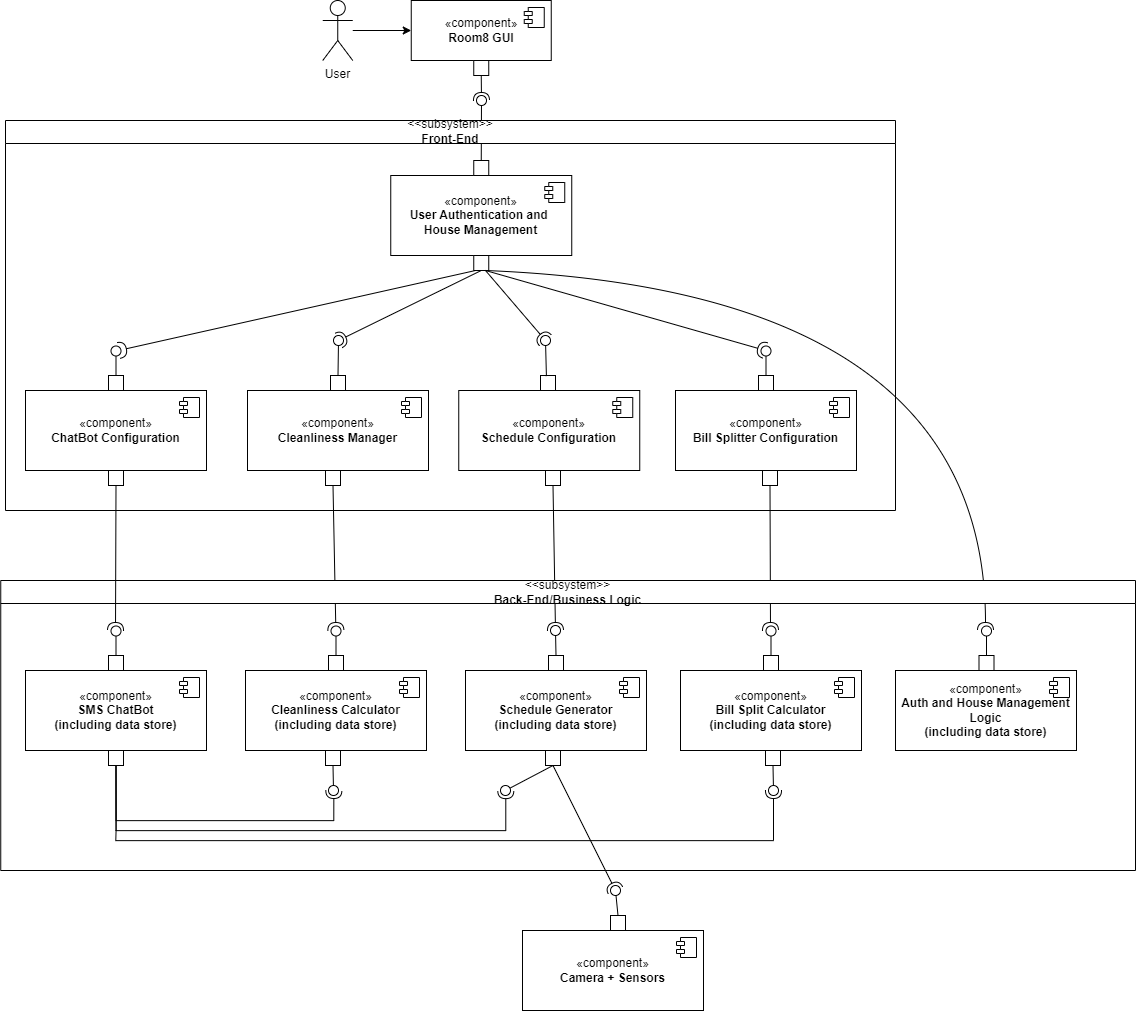
\includegraphics[width=\linewidth]{./img/component-diagram.png}
    \caption{Component Diagram}
    \label{fig: High level component diagram}
\end{figure}

\nsection{S.2 Functionality}

\begin{flushleft}
  \item \textbf{S.2.1 - User Authentication and House Management}
  	\begin{itemize}
  		\item \textbf{Functional Requirements:}
  		\begin{itemize}
  			\item \textbf{FR211:} The system shall allow users to create an account using their name, email, phone number, and password.
            \item \textbf{FR212:} The system shall allows users to log in to their account.
            \item \textbf{FR213:} The system shall allows users to log out of their account.
            \item \textbf{FR214:} The system shall allow users to create a home group using the home name, address, and number of roommates.
            \item \textbf{FR215:} The system shall allow users to invite other users to join their home group.
            \item \textbf{FR216:} The system shall allow users to view the list of users in their home group.
            \item \textbf{FR217:} The system shall allow users to remove users from their home group.
            \item \textbf{FR218:} The system shall allow users to leave their home group.
  		\end{itemize}
  		\item \textbf{Non-Functional Requirements:}
  		\begin{itemize}
  			\item \textbf{NFR211:} All data related to authentication must be encrypted in both transit and in storage.
  			\item \textbf{NFR212:} Error messages related to authentication should not disclose sensitive details such as "Incorrect Password".
  			\item \textbf{NFR213:} All data related to houses such as addresses and residents should be encrypted in transit and in rest.
  			\item \textbf{NFR214:} The system should be able to authenticate a user with a median response time of under 1 second.
  		\end{itemize}
  	\end{itemize}
  	\item \textbf{S.2.2 - ChatBot Configuration}
  	\begin{itemize}
  		\item \textbf{Functional Requirements:}
  		\begin{itemize}
  			\item \textbf{FR221:} The system shall allow users to configure the ChatBot settings to include or exclude messages corresponding to chore schedule, cleanliness manager, and bill splitter.
            \item \textbf{FR222:} The ChatBot shall send reminders to the group chat about upcoming chores and events in the schedule 2 days in advance.
            \item \textbf{FR223:} The ChatBot shall send notifications to the group chat about new shared living space cleanliness scores immediately after an event is added to the cleanliness manager page.
            \item \textbf{FR224:} The ChatBot shall send notifications to the group chat about new shared expenses added to the bill splitter page immediately after its addition.
            \item \textbf{FR225:} The system shall allow users to activate the ChatBot feature which will create combined groupchat including all the residents as well the bot itself.
  		\end{itemize}
  		\item \textbf{Non-Functional Requirements:}
  		\begin{itemize}
  			\item \textbf{NFR221}: The chatbot shall not disclose any sensitive information in its messages such as addresses or full names.
  			\item \textbf{NFR222}: The chatbot shall not send users too frequently to prevent annoying users.
  		\end{itemize}
  	\end{itemize}
  	\item \textbf{S.2.3 - Cleanliness Manager}
  	\begin{itemize}
  		\item \textbf{Functional Requirements:}
  		\begin{itemize}
            \item \textbf{FR231:} The system shall evaluate the cleanliness of the shared living space before and after a user enters and exits the space.
  			\item \textbf{FR232:} The system shall display the current cleanliness score of the shared living space.
            \item \textbf{FR233:} The system shall display the detected messes in the shared living space.
            \item \textbf{FR234:} The system shall allow users to view the history of cleanliness scores and detected messes.
        \end{itemize}
        \item \textbf{Non-Functional Requirements:}
        \begin{itemize}
            \item \textbf{NFR231:} The system shall not record users.
            \item \textbf{NFR232:} The system shall not capture images of users.
            \item \textbf{NFR233:} The system shall encrypt and securely store all images of homes.
            \item \textbf{NFR234:} Photos captured with the system will be in a quality high enough to differentiate objects within frame.
            \item \textbf{NFR235:} The system shall process image data in under 30 minutes.
            \item \textbf{NFR236:} The system shall not report false events which accuse someone of reducing the cleanliness score of an environment.
            \item \textbf{NFR237:} The system shall declare an instances of someone altering a room finished one there has been no activity in the room for a designated period of time.
  		\end{itemize}
  	\end{itemize}
  	\item \textbf{S.2.4 - Schedule Configuration}
  	\begin{itemize}
  		\item \textbf{Functional Requirements:}
  		\begin{itemize}
  			\item \textbf{FR241:} The system shall allow users to add a new chore to the schedule.
            \item \textbf{FR242:} The system shall allow users to add a new event to the schedule.
            \item \textbf{FR243:} The system shall allow users to input chore and event details (name, description, time, frequency, assigned users, etc.).
            \item \textbf{FR244:} The system shall allow users to edit and delete chores and events.
            \item \textbf{FR245:} The system shall allow users to view the schedule and mark chores as complete.
  		\end{itemize}
  		\item \textbf{Non-Functional Requirements:}
  		\begin{itemize}
  			\item \textbf{NFR241:} The calendar system shall store all calendar events in UTC
  			\item \textbf{NFR242:} The calendar system shall display all calendar events to users in their time zone. 
  			\item \textbf{NFR243:} The calendar system shall have a granularity of 5 minutes.
  			\item \textbf{NFR244:} The calendar system shall encrypt all events stored.
  		\end{itemize}
  	\end{itemize}
  	\item \textbf{S.2.5 - Bill Splitter Configuration}
  	\begin{itemize}
  		\item \textbf{Functional Requirements:}
  		\begin{itemize}
  			\item \textbf{FR251:} The system shall allow users to add a new expense to the bill splitter and notify the involved users.
            \item \textbf{FR252:} The system shall allow users to view what they owe other housemates.
            \item \textbf{FR253:} The system shall allow users to view what they owe others.
            \item \textbf{FR254:} The system shall allow users to mark expenses as paid.
            \item \textbf{FR255:} The system shall calculate debts in order to minimize the amount of transactions required between housemates.
  		\end{itemize}
  		\item \textbf{Non-Functional Requirements:}
  		\begin{itemize}
  			\item \textbf{NFR251:} The Bill Splitter system shall encrypt all events stored.
  			\item \textbf{NFR252:} The Bill Splitter shall allow users to record numerical values of prices with a granularity of two decimal places.

  		\end{itemize}
  	\end{itemize}
\end{flushleft}

\nsection{S.3 Interfaces}
At the time of writing, the application has not yet been implemented and no interfaces are being used.
Thus, S.3 Interfaces will be available in a future revision of this document.

\nsection{S.4 Detailed usage scenarios}

\nsubsection{S.4.1 User Creating an Account}
\begin{itemize}
    \item \textbf{Use Case:} UC1
    \item \textbf{Primary Actor:} New User
    \item \textbf{Precondition:} New User has a compatible device with internet access and opened the Room8 app.
    \item \textbf{Trigger:} New user wants to start using the app to manage their student home.

    \item \textbf{Main Success Scenario:}
    \begin{enumerate}
        \item User accesses the Room8 app.
        \item User selects the "Create Account" option.
        \item User fills in personal information (name, email, phone number, password).
        \item User submits the form.
        \item System validates the information and creates the account.
        \item System authenticates the user.
        \item System redirects the user to their dashboard.
    \end{enumerate}

    \item \textbf{Secondary Scenarios:}
    \begin{enumerate}
        \item[5.1] System is unable to create new user's account and informs the user of this error.
        \begin{enumerate}
            \item[5.1.1] System informs the user of the server error.
        \end{enumerate}
    \end{enumerate}

    \item \textbf{Success Postcondition:} New user is successfully registered and authenticated in the system. User is redirected to their dashboard with the option to create a home or join an existing one.
\end{itemize}

\nsubsection{S.4.2 User Logging Into an Account}
\begin{itemize}
    \item \textbf{Use Case:} UC1
    \item \textbf{Primary Actor:} User
    \item \textbf{Precondition:} User has an existing account and is not already logged in.
    \item \textbf{Trigger:} User wants to log into their account to use application features.

    \item \textbf{Main Success Scenario:}
    \begin{enumerate}
        \item User accesses the Room8 app.
        \item User selects the "Log In" option.
        \item User enters email and password.
        \item User submits the form.
        \item System authenticates the credentials and logs in the user.
        \item System redirects the user to their dashboard.
    \end{enumerate}

    \item \textbf{Secondary Scenarios:}
    \begin{enumerate}
        \item[5.1] User enters an invalid email and password combination.
            \begin{enumerate}
                \item[5.1.1] System informs the user of the invalid credentials.
            \end{enumerate}
        \item[5.2] System is unable to log into user's account and informs the user of this error.
        \begin{enumerate}
            \item[5.2.1] System informs the user of the server error.
        \end{enumerate}
    \end{enumerate}

    \item \textbf{Success Postcondition:} User is successfully logged into the system.
\end{itemize}

\nsubsection{S.4.3 User Logging Out of the System}
\begin{itemize}
    \item \textbf{Use Case:} UC1
    \item \textbf{Primary Actor:} User
    \item \textbf{Precondition:} User is already logged into their account.
    \item \textbf{Trigger:} User wants to log out of the system.

    \item \textbf{Main Success Scenario:}
    \begin{enumerate}
        \item User accesses the main menu of the Room8 app.
        \item User selects the "Log Out" option.
        \item System prompts for confirmation.
        \item User confirms the action.
        \item System logs the user out and redirects to the login screen.
    \end{enumerate}

    \item \textbf{Secondary Scenarios:}
    \begin{enumerate}
        \item[4.1] User cancels the log out action.
    \end{enumerate}

    \item \textbf{Success Postcondition:} User is successfully logged out of the system.
\end{itemize}

\nsubsection{S.4.4 User Creates a Home}
\begin{itemize}
    \item \textbf{Use Case:} UC2
    \item \textbf{Primary Actor:} User
    \item \textbf{Secondary Actor:} User's roommates
    \item \textbf{Precondition:} User is logged in and has no existing home.
    \item \textbf{Trigger:} User wants to create a home to manage their living situation with their roommates.

    \item \textbf{Main Success Scenario:}
    \begin{enumerate}
        \item User navigates to their dashboard.
        \item User selects the "Create Home" option.
        \item User enters home details (home name, address, etc.).
        \item User sends invitations to housemates by entering their email addresses.
        \item System sends email notifications to invited users.
        \item Invited users accept or decline the invitation.
    \end{enumerate}

    \item \textbf{Secondary Scenarios:}
    \begin{enumerate}
        \item[4.1] User does not invite any housemates and chooses to invite them later. 
    \end{enumerate}

    \item \textbf{Success Postcondition:} User has successfully created a home and invited housemates to join.
\end{itemize}

\nsubsection{S.4.5 User Joins a Home}
\begin{itemize}
    \item \textbf{Use Case:} UC2
    \item \textbf{Primary Actor:} User
    \item \textbf{Secondary Actor:} User's roommates
    \item \textbf{Precondition:} User is logged in and has no existing home.
    \item \textbf{Trigger:} User wants to join their home's existing group.

    \item \textbf{Main Success Scenario:}
    \begin{enumerate}
        \item User receives an email invitation to join a home.
        \item User clicks on the provided link in the invitation.
        \item System redirects user to the Room8 app.
        \item User logs in.
        \item User confirms their decision to join the home.
        \item System adds the user to the home group.
        \item System notifies the housemates of the new addition.
    \end{enumerate}

    \item \textbf{Secondary Scenarios:}
    \begin{enumerate}
        \item[4.1] User does not have an account and is prompted to create one.
        \item[5.1] User is unable to join the home and is informed of this error.
        \item[5.2] User declines the prompt and is not added to the home.
    \end{enumerate}

    \item \textbf{Success Postcondition:} User has join home alongside their housemates.
\end{itemize}

\nsubsection{S.4.6 User Leaves a Home}
\begin{itemize}
    \item \textbf{Use Case:} UC2
    \item \textbf{Primary Actor:} User
    \item \textbf{Secondary Actor:} User's roommates
    \item \textbf{Precondition:} User is logged in and has an existing home.
    \item \textbf{Trigger:} User wants to leave the home attached to their account.

    \item \textbf{Main Success Scenario:}
    \begin{enumerate}
        \item User navigates to their Home settings.
        \item User chooses the "Leave Home" option.
        \item System prompts for confirmation.
        \item User confirms the action.
        \item System removes the user from the home group.
        \item System redirects the user to their dashboard.
        \item System notifies the housemates of the user's departure.
    \end{enumerate}

    \item \textbf{Secondary Scenarios:}
    \begin{enumerate}
        \item[4.1] User aborts leaving the home and remains in the group.
    \end{enumerate}

    \item \textbf{Success Postcondition:} User has left the home and is no longer associated with the group. User is in the dashboard page with the option to create a home or join an existing one.
\end{itemize}

\nsubsection{S.4.7 User Schedules a Chore}
\begin{itemize}
    \item \textbf{Use Case:} UC3
    \item \textbf{Primary Actor:} User
    \item \textbf{Secondary Actor:} User's roommates
    \item \textbf{Precondition:} User is logged in and has an existing home.
    \item \textbf{Trigger:} User wants to schedule a chore amongst housemates to assign responsibilities. 

    \item \textbf{Main Success Scenario:}
    \begin{enumerate}
        \item User navigates to the "Schedule” section.
        \item User selects "Add New Chore".
        \item User inputs chore details (name, description, time, frequency, etc.).
        \item User assigns housemates to the chore.
        \item User confirms chore creation.
        \item System saves the chore and adds it to the schedule.
        \item System notifies housemates of the new chore.
    \end{enumerate}

    \item \textbf{Secondary Scenarios:}
    \begin{enumerate}
        \item[3.1] User does input all required chore details correctly.
        \begin{enumerate}
            \item[3.1.1] System prompts the user to fill in all required fields.
        \end{enumerate}
        \item[5.1] User cancels the chore creation.
    \end{enumerate}

    \item \textbf{Success Postcondition:} New chore is added to the schedule and housemates are notified. Housemates are reminded of the chore when it is approaching.
\end{itemize}

\nsubsection{S.4.8 User Edits a Chore}
\begin{itemize}
    \item \textbf{Use Case:} UC3
    \item \textbf{Primary Actor:} User
    \item \textbf{Secondary Actor:} User's roommates
    \item \textbf{Precondition:} User is logged in and has an existing home. User has an existing chore.
    \item \textbf{Trigger:} User wants to update chore details.

    \item \textbf{Main Success Scenario:}
    \begin{enumerate}
        \item User navigates to the "Schedule” section.
        \item User selects a scheduled chore.
        \item User chooses the "Edit" option.
        \item User modifies the chore details (name, description, time, frequency, assigned users, etc.).
        \item User confirms the changes.
        \item System updates the chore and notifies relevant housemates.
    \end{enumerate}

    \item \textbf{Secondary Scenarios:}
    \begin{enumerate}
        \item[5.1] User cancels the chore creation.
    \end{enumerate}

    \item \textbf{Success Postcondition:} Chore is updated and housemates are notified of the updated chore.
\end{itemize}

\nsubsection{S.4.9 User Completes a Chore}
\begin{itemize}
    \item \textbf{Use Case:} UC3
    \item \textbf{Primary Actor:} User
    \item \textbf{Precondition:} User is logged in and has an existing home. User has an existing chore.
    \item \textbf{Trigger:} User has completed their chore duties and wants to update the schedule to reflect their completed duties.

    \item \textbf{Main Success Scenario:}
    \begin{enumerate}
        \item User navigates to the "Schedule” section.
        \item User selects a chore assigned to them.
        \item User is able to see chore details, description, and due date.
        \item User chooses the "Complete" option.
        \item System marks the chore as complete and updates the chore history.
    \end{enumerate}

    \item \textbf{Success Postcondition:} Chore is completed and system displays the next upcoming undone chore. Chore history reflects list of completed chores in the home.
\end{itemize}

\nsubsection{S.4.10 User Schedules an Event}
\begin{itemize}
    \item \textbf{Use Case:} UC3
    \item \textbf{Primary Actor:} User
    \item \textbf{Secondary Actor:} User's roommates
    \item \textbf{Precondition:} User is logged in and has an existing home.
    \item \textbf{Trigger:} User wants to schedule the use of a shared living space and notify housemates.

    \item \textbf{Main Success Scenario:}
    \begin{enumerate}
        \item User navigates to the "Schedule" section.
        \item User selects the "Add Event" option.
        \item User inputs event details (date, time, description).
        \item User sets reminders or notifications.
        \item User confirms the event creation.
        \item System adds the event to the users' schedule.
    \end{enumerate}

    \item \textbf{Secondary Scenarios:}
    \begin{enumerate}
        \item[3.1] User does not input all required event details correctly.
        \begin{enumerate}
            \item[3.1.1] System prompts the user to fill in all required fields.
        \end{enumerate}
        \item[5.1] User cancels the event creation.
    \end{enumerate}

    \item \textbf{Success Postcondition:} New event is added to the schedule and housemates are notified. Housemates are able to view event in the schedule. Housemates are reminded of the event when it is approaching.
\end{itemize}

\nsubsection{S.4.11 User Views Chores Or Events}
\begin{itemize}
    \item \textbf{Use Case:} UC3
    \item \textbf{Primary Actor:} User
    \item \textbf{Precondition:} User is logged in and has an existing home.
    \item \textbf{Trigger:} User wants to view the history of completed and pending chores.

    \item \textbf{Main Success Scenario:}
    \begin{enumerate}
        \item User navigates to the "Schedule” section.
        \item User selects the "Chore History" option.
        \item System displays a list of completed and pending chores.
        \item User can filter or search through the history.
    \end{enumerate}

    \item \textbf{Secondary Scenarios:}
    \begin{enumerate}
        \item[3.1] User does not have any completed or pending chores.
        \begin{enumerate}
            \item[3.1.1] System informs the user that there are no chores to display.
        \end{enumerate}
    \end{enumerate}

    \item \textbf{Success Postcondition:} User is able to view the history of completed and pending chores. User is able to filter and search through the history.
\end{itemize}

\nsubsection{S.4.12 User Adds an Expense}
\begin{itemize}
    \item \textbf{Use Case:} UC4
    \item \textbf{Primary Actor:} User
    \item \textbf{Secondary Actor:} User's roommates
    \item \textbf{Precondition:} User is logged in and has an existing home.
    \item \textbf{Trigger:} User wants to add a shared expense to the house and split the bill between housemates to keep track of who owes what.

    \item \textbf{Main Success Scenario:}
    \begin{enumerate}
        \item User navigates to the “Bill Splitter” section.
        \item User selects the "Add Expense" option.
        \item User enters the total expense amount and description.
        \item User selects which housemates are responsible for the expense.
        \item User confirms the expense.
        \item System splits the expense and notifies the involved users.
    \end{enumerate}

    \item \textbf{Secondary Scenarios:}
    \begin{enumerate}
        \item[3.1] User does not input all required expense details correctly.
        \begin{enumerate}
            \item[3.1.1] System prompts the user to fill in all required fields.
        \end{enumerate}
        \item[5.1] User cancels the expense creation.
    \end{enumerate}

    \item \textbf{Success Postcondition:} New expense is added. Expense is split between housemates and housemates are notified. Housemates are able to view the expense in the bill splitter section.
\end{itemize}

\nsubsection{S.4.13 User Views Expenses}
\begin{itemize}
    \item \textbf{Use Case:} UC4
    \item \textbf{Primary Actor:} User
    \item \textbf{Secondary Actor:} User's roommates
    \item \textbf{Precondition:} User is logged in and has an existing home. Home has existing expenses.
    \item \textbf{Trigger:} User wants to view the history of expenses and bills in the house. User wants to see who owes them money. User wants to see who they owe money to.  

    \item \textbf{Main Success Scenario:}
    \begin{enumerate}
        \item User navigates to the "Bill Splitter" section.
        \item User selects the "Expense History" option.
        \item System displays a list of past payments and outstanding bills.
        \item User can filter the history by type or amount.
    \end{enumerate}

    \item \textbf{Success Postcondition:} User is able to see current list of housemates and their outstanding bills between themselves and the other housemates. User is able to filter and search through the history of shared expenses.
\end{itemize}

\nsubsection{S.4.14 User Pays an Expense}
\begin{itemize}
    \item \textbf{Use Case:} UC4
    \item \textbf{Primary Actor:} User
    \item \textbf{Secondary Actor:} User's roommates
    \item \textbf{Precondition:} User is logged in and has an existing home. User has an existing unpaid bill with one of the housemates.
    \item \textbf{Trigger:} User wants to mark an expense between themselves and another housemate as paid and update the payment status.

    \item \textbf{Main Success Scenario:}
    \begin{enumerate}
        \item User navigates to the "Bill Splitter" section.
        \item User selects their profile's bills.
        \item User selects an unpaid bill.
        \item User marks the bill as paid.
        \item System updates the payment status and recalculates debts.
        \item System notifies other housemates about the payment status.
    \end{enumerate}

    \item \textbf{Success Postcondition:} Expenses are updated and expense log reflects expense transactions. Debts are recalculated to facilitate the least amount of transactions between housemates.
\end{itemize}

\nsubsection{S.4.15 User Views Cleanliness Score}
\begin{itemize}
    \item \textbf{Use Case:} UC5
    \item \textbf{Primary Actor:} User
    \item \textbf{Precondition:} User is logged in and has an existing home. Home has cleanliness detector setup.
    \item \textbf{Trigger:} User wants to view current cleanliness score of the shared living space and latest usage.

    \item \textbf{Main Success Scenario:}
    \begin{enumerate}
        \item User navigates to the “Cleanliness Management” section.
        \item System displays the current cleanliness score and detected messes.
        \item User selects another user to view their cleanliness score.
        \item System displays the selected user’s cleanliness score and pending tasks associated with their shared living space usage.
    \end{enumerate}

    \item \textbf{Secondary Scenarios:}
    \begin{enumerate}
        \item[3.1] User does not have any detected messes.
        \begin{enumerate}
            \item[3.1.1] System informs the user that there are no detected messes.
        \end{enumerate}
    \end{enumerate}

    \item \textbf{Success Postcondition:} User is able to view the current cleanliness score of the shared living space. User is able to view detected messes and cleanliness score of other housemates.
\end{itemize}

\nsubsection{S.4.16 Add ChatBot to Group Chat}
\begin{itemize}
    \item \textbf{Use Case:} UC6
    \item \textbf{Primary Actor:} User
    \item \textbf{Secondary Actor:} User's roommates, ChatBot
    \item \textbf{Precondition:} User is logged in and has an existing home.
    \item \textbf{Trigger:} User wants to recieve SMS messages regarding cleanliness, chores, expenses, and events in the shared living space in a group chat outside of the Room8 app.

    \item \textbf{Main Success Scenario:}
    \begin{enumerate}
        \item User navigates to the “Chat Management” section.
        \item User selects the option to add a ChatBot to their house group chat.
        \item User inputs notification and reminder settings.
        \item System generates an SMS numbers and instructions to add the ChatBot to the group chat.
        \item User adds the ChatBot to the group chat.
        \item The ChatBot sends a welcome message to the group.
    \end{enumerate}

    \item \textbf{Secondary Scenarios:}
    \begin{enumerate}
        \item[5.1] Users fail to add the ChatBot to the group chat.
        \begin{enumerate}
            \item[5.1.1] System informs the user that the ChatBot has not been added.
        \end{enumerate}
    \end{enumerate}

    \item \textbf{Success Postcondition:} User is able to recieve SMS messages regarding cleanliness, chores, expenses, and events in the shared living space in a group chat outside of the Room8 app.
\end{itemize}

\nsection{S.5 Prioritization}

\begin{table}[H]
    \flushleft
    \begin{tabularx}{\textwidth}{|>{\raggedright}X|>{\raggedright}X|>{\raggedright}X|X|}
    \hline
    \textbf{Requirement ID} & \textbf{Description} & \textbf{MoSCoW Classification} & \textbf{Reasoning} \\ \hline
    F211, FR212, FR213 & Account Authentication & Must have & App features require users to be authenticated to use. \\ \hline

    F214, FR215, FR216, FR217, FR218 & House Management & Must have & App features all require users to be part of a home. \\ \hline

    FR221 & ChatBot Configuration & Could have & Allows users to customize notifications to their needs. \\ \hline

    FR222, FR223, FR224 & ChatBot Notification Messages & Should have & Allows users to conveniently recieve notifications in a shared setting. \\ \hline

    FR231 & Cleanliness Evaluation After Usage & Should have & Removes frequent point of friction in living spaces for users. \\ \hline

    FR232 & Cleanliness Score & Could have & Summarizes detected messes into a score. \\ \hline

    FR233 & Cleanliness Detected Messes & Should have & Very important to assigning responsibilities to users. \\ \hline

    FR234, FR235 & User Cleanliness and History & Could have & Provides history for user's performance. \\ \hline
\end{tabularx}
\caption{Requirement Specifications Part 1}
\end{table}
\begin{table}[H]
    \flushleft
    \begin{tabularx}{\textwidth}{|>{\raggedright}X|>{\raggedright}X|>{\raggedright}X|X|}
    \hline
    \textbf{Requirement ID} & \textbf{Description} & \textbf{MoSCoW Classification} & \textbf{Reasoning} \\ \hline
    FR241, FR242, FR243 & Chore \& Event Management & Must have & Scheduling chores is an essential feature in student housing. \\ \hline

    FR244 & Edit Chore \& Event & Could have & Allows users update their schedule with ease. \\ \hline

    FR245 & Marking Chores Complete & Should have & Provides users with a way to track completed chores. \\ \hline

    FR251, FR252, FR253, FR254 & Add \& View Split Bills & Must have & Essential feature in managing shared resources in student housing. \\ \hline

    FR255 & Calculate Least Transactions & Could have & Convenient feature which makes users lives easier. \\ \hline
    \end{tabularx}
    \caption{Requirement Specifications Part 2}
\end{table}

\nsection{S.6 Verification and acceptance criteria}
\textbf{Functional Requirements}\\
In order to validate functional requirements, a systematic approach will be implemented. Features will be validated against criteria made by developers, testers and stakeholders. Using the criteria unit and intergration tests will be developed for consistency. \\
\\
\textbf{Non-Functional Requirements}\\
\textbf{Tests for User Account Mangement}
\begin{itemize}
    \item Account Creation Flow
    	\begin{itemize}
    		\item  A new user trying to create an account, when sign-up process is started 				they then should be able to enter details and create account with details being stored in secured manner. [NFR211].
		\end{itemize}    	
    \item Error Handling For Incorrect Information
    	\begin{itemize}
    		\item  A user trying to login to an account, when login process is started 				and they make mistake, (eg. enter wrong password), no information pertaining to sensitive detail should be displayed. [NFR212].
		\end{itemize}
	\item Account Authentication
    	\begin{itemize}
    		\item  A user trying to login and authenticating their account should be able to have account authenticated must be done in less than 1 second. [NFR214]. \\
		\end{itemize}		
\textbf{Tests for Calendar Interactions}\\

		\item Calendar Event Creation
    	\begin{itemize}
    		\item  A user who has logged on to the application will create an event then change the time 1 increment above the original time on the calendar and the system will store the event in UTC while the event will show up on the user's device in the user's respective timezone. [NFR241, NFR242, NFR243].
		\end{itemize}
\end{itemize}



%===============================================================
\chapter*{Project}
\addcontentsline{toc}{chapter}{Project book}
\setcounter{mtc}{4}
\minitoc% Creating an actual minitoc
%===============================================================


\nsection{P.1 Roles and personnel}
Note: Roles that cannot be assigned to multiple people are denoted with a \textbf{*}\\
\newline Role Switching: Roles can be switched and reassigned with an informal verbal agreement with the exception of Developer Liaison, which requires the previous liaison to notify all external contacts of the change in point of contact.\\
\newline\textbf{Project Manager*: }Responsible for making sure Room8 project is operating smoothly. Ensures resources being allocated efficiently, issues on Github are being solved, project tasks are being tracked and chairs team meetings.\\
\\
\textbf{Application Developer: }Responsible for developing the Room8 application which will be the main point of interaction between users and projects. Tasks this role is responsible for also include API design and UI/UX design.\\
\\
\textbf{DevOps Engineer: }Responsible for creating and maintaining CI/CD pipelines to ensure the latests builds are deployed to the production environment.\\
\\
\textbf{Cloud Engineer: }Responsible for creating designing, implementing, and managing any required cloud-based solutions needed for the project. These include cloud based storage containers and application deployments.\\
\\
\textbf{Hardware Specialist: }Responsible for researching and implementing any required hardware solutions as well integrating them with the application and other software components.\\
\\
\textbf{AI Engineer: }Responsible for researching, implementing, and tuning any required AI models needed for implementation.\\
\\
\textbf{Developer Liaison*: }The point of contact between project developers and stakeholders. The Liaison will be responsible for scheduling non-developer meetings and responding to questions from stakeholders. \\
\\

\nsection{P.2 Imposed technical choices}
Due to time constraints, project requirements, and the skill sets of the team's current developers, some imposed technical choices are:
\begin{itemize}
\item \textbf{JS/TS Application Framework}. This is due to JS/TS being known by a majority of the developers and it having a plethora of existing, well-documented frameworks.
\item \textbf{AWS Cloud Services}. AWS is the leading cloud platform and one which our developers have experience developing in.
\item \textbf{Google Calendar and Google OAuth}. Google provides very generous free tiers for their OAuth and cloud solutions.

\end{itemize}

\nsection{P.3 Schedule and milestones}
\begin{itemize}
    \item \textbf{Milestone 1 (September 23rd) - Initial concept and development plan}
    \begin{itemize}
        \item Deliverable: Problem Statement and Goals
        \item Deliverable: Development Plan
    \end{itemize}

    \item \textbf{Milestone 2 (October 11) - Requirements}
    \begin{itemize}
        \item Deliverable: SRS
    \end{itemize}

    \item \textbf{Milestone 3 (October 23) - Hazard Analysis}
    \begin{itemize}
        \item Deliverable: Hazard Analysis Report
    \end{itemize}

    \item \textbf{Milestone 4 (November 1st) - V\&V Plan}
    \begin{itemize}
        \item Deliverable: V\&V Plan
    \end{itemize}

    \item \textbf{Milestone 5 (Within November 11-22) - PoC demonstration}
    \begin{itemize}
        \item Event: Informal Project Demonstration
        \item Goal: Core features functional
    \end{itemize}

    \item \textbf{Milestone 6 (January 15) - Design Documents}
    \begin{itemize}
        \item Deliverable: Software Architecture Document
        \item Deliverable: Detailed Design Document
    \end{itemize}

    \item \textbf{Milestone 7 (within February 3-14) - Revision 0 \& Project completion}
    \begin{itemize}
        \item Goal: Project is Complete and Functional
    \end{itemize}

    \item \textbf{Milestone 8 (March 7th) - Verify \& Validate}
    \begin{itemize}
        \item Deliverable: V\&V Report
        \item Goal: Project meets all requirements outlined in the SRS and V\&V Plan
    \end{itemize}

    \item \textbf{Milestone 9 (within March 24-30) - Final demonstration}
    \begin{itemize}
    	\item Event: Final Project Demonstration
    	\item Goal: Unmet requirements from Milestone 8 are resolved
    \end{itemize}

    \item \textbf{Milestone 10 (April) - Project EXPO demonstration}
    \begin{itemize}
        \item Deliverable: Project Poster
        \item Event: Project Expo
    \end{itemize}

    \item \textbf{Milestone 11 (April 2nd) - Final documentation}
    \begin{itemize}
        \item Deliverable: Final Problem Statement
        \item Deliverable: Development Plan
        \item Deliverable: PoC Plan
        \item Deliverable: Updated Requirements document
        \item Deliverable: V\&V Plan
        \item Deliverable: V\&V Report
        \item Deliverable: User Guide
        \item Deliverable: Project Source Code
    \end{itemize}
\end{itemize}

\nsection{P.4 Tasks and deliverables}

\noindent
\textbf{Milestone 1}\\
Details:
\begin{itemize}
\item Abstract the problem to be solved and characterize it in terms of inputs and outputs.
\item Research the importance of the problem and possible stakeholders.
\item Establish measurable goals and selling points of the product.
\item Discuss team availabilities, roles, and communication strategies.
\item Discuss potential workflows, technologies, and coding styles.
\item Establish plan and timeline for a PoC.
\end{itemize}
Expected Outcomes:
\begin{itemize}
\item Problem Statement and Goals.
\item Development Plan.
\item Team Charter.
\item Git Repository and Online Project Board.
\end{itemize}
\textbf{Milestone 2}\\
Details:
\begin{itemize}
\item Revisit problem statement.
\item Revisit project goals.
\item Revisit stakeholders.
\item Gather user requirements.
\item Establish functional and non-functional requirements.
\item Establish project use cases.
\item Establish system constraints.
\item Establish expected system environment and assumptions.
\end{itemize}
Expected Outcomes:
\begin{itemize}
\item SRS Document.
\end{itemize}
\textbf{Milestone 3}\\
Details:
\begin{itemize}
\item Explore possible data privacy issues in the project.
\item Explore scenarios where user's provide incorrect input.
\item Explore scenarios where the system isn't running in it's ideal environment.
\item Explore hazard mitigation strategies for the above scenarios.
\end{itemize}
Expected Outcomes:
\begin{itemize}
\item Hazard Analysis Document.
\item Improvement of project security, data privacy, and error handling.
\end{itemize}
\textbf{Milestone 4}\\
Details:
\begin{itemize}
\item Analyze features and determine appropriate test plan.
\item Establish test plan for non-functional requirements.
\item Establish metrics and success criteria for validation.
\item Establish a timeline for V\&V.
\item Determine if manual testing is required.
\item Trace tests to functional requirements.
\end{itemize}
Expected Outcomes:
\begin{itemize}
\item V\&V Plan.
\item Automated testing suite using CI/CD tools.
\end{itemize}
\textbf{Milestone 5}\\
Details:
\begin{itemize}
\item Establish scope of the PoC demonstration.
\item Prepare presentation materials such as documents or slides. TBD based on demonstration format.
\item Establish core use cases for the PoC demonstration.
\item Rehearse PoC demonstration.
\end{itemize}
Expected Outcomes:
\begin{itemize}
\item Feedback from stakeholders.
\item Revised project goals and priorities.
\item Feasibility Validation.
\item Identification of Risks.
\end{itemize}
\textbf{Milestone 6}\\
Details:
\begin{itemize}
\item Discuss and establish design to satisfy functional and non-functional requirements.
\item Design system modules and architecture. Associate system concerns to system modules.
\item Create test cases.
\end{itemize}
Expected Outcomes:
\begin{itemize}
\item Software Architecture Document.
\item Detailed Design Document.
\end{itemize}
\textbf{Milestone 7}\\
Details:
\begin{itemize}
\item Identify tasks (issues) to be finished alongside their deadlines.
\item Identify task ownership and distribute tasks.
\item Write system code and build the software module.
\item Create any custom hardware components required.
\item Connect software module to the hardware (if required).
\item Perform User Acceptance Tests.
\end{itemize}
Expected Outcomes:
\begin{itemize}
\item Functional Application.
\item Any Necessary Hardware Components.
\end{itemize}
\textbf{Milestone 8}\\
Details:
\begin{itemize}
\item Apply the procedure outlined in the V\&V plan.
\item Create additional tests and testing code needed to verify unverified requirements.
\item Document unexpected results.
\item Document what requirements haven't been met and develop an actual plan to meet them.
\end{itemize}
Expected Outcomes:
\begin{itemize}
\item V\&V Report.
\item Resolution of any unmet requirements.
\end{itemize}
\textbf{Milestone 9 \& Milestone 10 - Project Demonstrations}\\
Details:
\begin{itemize}
\item Finalize list of project selling points.
\item Rehearse project demo and establish primary, secondary, and tertiary use cases.
\end{itemize}
Expected Outcomes:
\begin{itemize}
\item Project Poster.
\item Project Showcase Video.
\end{itemize}
\textbf{Milestone 11}\\
Details:
\begin{itemize}
\item Revisit all previously created documentation and make any necessary corrections.
\item Record steps needed to install and setup the system from a user perspective.
\end{itemize}
Expected Outcomes:
\begin{itemize}
\item Revised Project Documentation.
\item User Guide.
\end{itemize}
\nsection{P.5 Required technology elements}

\textbf{Camera} \\
A camera is used for the systems cleanliness detection aspect. A camera takes pictures for comparing the state of the shared space.\\
\\
\textbf{Motion Sensor}\\
A sensor is also used for the systems cleanliness detection aspect. The sensor detects movement which will work in unison with the camera to take pictures of the shared space.\\
\\
\textbf{Third Party Calendar API}\\
Room8's scheduler requires a calendar component where user's can book and view events and chores in a calendar. Implementing a calendar API from scratch can prove difficult and there are already many existing solutions.\\
\\
\textbf{Secure Database}\\
Users create accounts for Room8 where user and home information is stored on a secure database where sensitive information such as credentials are stored and individuals are able to change and delete accounts.\\
\\
\textbf{Third Party OAuth Service}\\
Users will sign in securely without risk of data leaks and malicious connections.\\
\\
\textbf{SMS Message Service}\\
Room8's ChatBot SMS will send messages to users using a third party messaging system that has connection to the Room8 application to send warnings and information of shared space.\\


\nsection{P.6 Risks and mitigation analysis}

\textbf{Machine Learning Model Training}\\
Finding enough data to train the machine learning algorithm to detect when a mess has been made and what detect what is altered or added in the space. Sensitivity to slight changes such as lighting is another risk with the machine learning algorithm approach. An alternative to adapt this scenario would be to use image differencing to detect changes in environment.\\
\\
\textbf{User Identification}\\
Being able to detect which user is using the shared space through the camera is a major risk. The program may not be supplied with enough information to identity which user is currently using the space. In order to work around this the program could get individuals to submit to the application that they are now using the space.\\
\\
\textbf{Scope Creep}\\
Unclear requirements and adding too many elements to the scope of the project will result in not delivering on features that are listed to be part of the application and lower quality of core functionality due to time being strain. A revisal of requirements by making requirements and functionality of system clear and concise and developing a prioritization list would mitigate the risk of scope creep.


\nsection{P.7 Requirements process and report}
\textbf{Requirements Elicitation}\\
For the elicitation of our requirements, we were able to discuss with our peers, who live in shared living situations, and took inspiration from our own experience as students who also have the need for an application like Room8.\\
\\
\textbf{Requirements Analysis}\\
The analysis of the requirements was completed as part of the problem statement and goals. As a group, we took the goals that we created in that part of the project and extracted them as functional requirements. Additionally, there were non-functional requirements that were mistakenly added as goals in revision 0 of that document, which gave us a basis for the specification.\\
\\\\\\
\textbf{Requirements Specification}\\
Evidently, the requirements specification are described in our Software Requirements Specification (this document itself). They will remain as the project continues and will be updated accordingly. \\
\\
\textbf{Requirements Validation}\\
The requirements validation will take place at two different stages of the project. First, they will be validated at the point of the PoC demo, where we will determine if the scope of the project is appropriate and we can pivot (add/reduce requirements) at that point. Furthermore, the final requirements will be assessed when the project is complete and demonstrated at the end of the Winter semester.\\
\\
\textbf{Requirements Management}\\
As previously mentioned, additional requirements will be made as necessary in this document and appended iteratively.

    \newpage{}
\section*{Appendix --- Reflection}

The information in this section will be used to evaluate the team members on the
graduate attribute of Lifelong Learning.  

% \input{../Reflection.tex}

\begin{enumerate}
  \item \textbf{What went well while writing this deliverable?} \\
When writing this deliverable the formatting of the document went smoothly. With the example texts and functions made intially on the example .tex document we were able to format the document to the requirements given to ensure a readable document. Also, the sectioning and table of content makes the document easy to navigate and the sections are ordered in a way that makes sense. This way when looking for a section in the requirement it is easy to find. Seeing as this is a cruicial document which will be referred to multiple times throughout the project, the setup, and readability of the document is integral.
  \item \textbf{What pain points did you experience during this deliverable, and how did
  you resolve them?}\\
A major pain point of this deliverable was we did not know which SRS format to use as there were three different ones given. Initially we went with the SRS with no label (scientific computation) but then realized after checking lecture slides this was the wrong one. We then had to start over using the proper template. This caused us to fall behind schedule.
  \item \textbf{How many of your requirements were inspired by speaking to your
  client(s) or their proxies (e.g. your peers, stakeholders, potential users)?}\\
Almost half of our requirements were inspired by talking to peers and just personal experience from each of us. We fall under the group of stakeholders (students living off campus) and we choose to make this project from scratch because we have experienced the pain points covered in the requirements much like how our peers have as well. We did this through casual conversation with our classmates and friends alike.
  \item \textbf{Which of the courses you have taken, or are currently taking, will help
  your team to be successful with your capstone project.}\\
A course all of us have taken is SFWRENG 3RA3 Software Requirements course which is meant exactly for this deliverable. It went over key software requirement document components and helped us form this document. Another course that will help later down the line is COMPSCI 3ML3 which 4 of the 5 group members are taking. This will help in developing and learning about the machine learning algorithm.
  \item \textbf{What knowledge and skills will the team collectively need to acquire to
  successfully complete this capstone project?  Examples of possible knowledge
  to acquire include domain specific knowledge from the domain of your
  application, or software engineering knowledge, mechatronics knowledge or
  computer science knowledge.  Skills may be related to technology, or writing,
  or presentation, or team management, etc.  You should look to identify at
  least one item for each team member.}\\
There are about 4 key concepts the team will collectively need to acquire in order to successfully complete the project. The first is knowledge of machine learning. This will help us train the model and learn how the algorithm will work. Another is software testing because this will help us test the system and see if it's working correctly and properly under edge cases. Data privacy is also important for our project because without protecting user information the project will not be viable.
  \item \textbf{For each of the knowledge areas and skills identified in the previous
  question, what are at least two approaches to acquiring the knowledge or
  mastering the skill?  Of the identified approaches, which will each team
  member pursue, and why did they make this choice?}\\
For all knowledge areas listed above, there are courses available at McMaster to learn these skills. However, because we can not take all these courses because of elective restrictions, there are textbooks and online texts and videos available covering these topics. This will be the go to for most group members however some group memebrs already have experience and knowledge in these domains whether its from previous work experiences or courses taken. We will teach each other and learn together and take advantage of each others strengths to ensure progress in each field. 
\end{enumerate}

\newpage{}
\section*{Appendix --- Citations}
[1] “How to get along with your roommate,” Centre for Innovation in Campus Mental Health, \href{https://campusmentalhealth.ca/infosheets/how-to-get-along-with-your-roommate/}{https://campusmentalhealth.ca/infosheets/how-to-get-along-with-your-roommate/} (accessed Oct. 11, 2024).

%===============================================================
\end{document}
%===============================================================